\documentclass[nooutcomes]{ximera}
\usepackage{booktabs}
%% handout
%% space
%% newpage
%% numbers
%% nooutcomes

\renewcommand{\outcome}[1]{\marginpar{\null\vspace{2ex}\scriptsize\framebox{\parbox{0.75in}{\begin{raggedright}\textbf{P\arabic{problem} Outcome:} #1\end{raggedright}}}}}

\renewenvironment{freeResponse}{
\ifhandout\setbox0\vbox\bgroup\else
\begin{trivlist}\item[\hskip \labelsep\bfseries Solution:\hspace{2ex}]
\fi}
{\ifhandout\egroup\else
\end{trivlist}
\fi}

\newcommand{\RR}{\mathbb R}
\renewcommand{\d}{\,d}
\newcommand{\dd}[2][]{\frac{d #1}{d #2}}
\renewcommand{\l}{\ell}
\newcommand{\ddx}{\frac{d}{dx}}
\everymath{\displaystyle}
\newcommand{\dfn}{\textbf}
\newcommand{\eval}[1]{\bigg[ #1 \bigg]}


\title{Breakout Session 20 Solutions}

\begin{document}
\begin{abstract}
\end{abstract}
\maketitle

% \section{Learning Outcomes}
% \label{section:learning-outcomes}
% The following outcomes are \emph{not an exhaustive} list of the skills you will need to develop and integrate for demonstration on quizzes and exams.
% This list is meant to be a starting point for conversation (with your Lecturer, Breakout Session Instructor, and fellow learners) for organizing your knowledge and monitoring the development of your skills.

% \begin{itemize}
%   \item Determine whether Rolle’s Theorem and/or MVT can be applied. 
%   \item Find the values guaranteed by Rolle’s Theorem or MVT. 
%   \item Use MVT to solve word problems. 
%   \item Compare and contrast the IVT, MVT, and Rolle’s Theorem.
%   \item Understand what the MVT tells us. 
%   \item Identify calculus ideas which are consequences of the MVT. 

%   \item Determine if a form is indeterminate.
%   \item Define an indeterminate form.
%   \item Convert indeterminate forms to $0/0$ or $\infty/\infty$.
%   \item State L'H\^{o}pital's Rule and identify when it can be used.
%   \item Use L'H\^{o}pital's Rule to find limits. 
%   \item Recall how to find limits for forms that are not indeterminate. 

% \end{itemize}
% \newpage

\begin{problem}
  \outcome{Determine whether Rolle’s Theorem and/or MVT can be applied.}
  \outcome{Understand what the MVT tells us.}
  \outcome{Identify calculus ideas which are consequences of the MVT.}
  Given the four functions on the interval $[1, 5]$, answer the questions below.
  \begin{image}
    \includegraphics[scale = 0.4]{Images/"Graph of four functions".png}
  \end{image}
  \begin{itemize}
    \item[(i)]
      List the function that satisfies (or functions that satisfy) the conditions of the Mean Value Theorem on $[1, 5]$.
      \begin{freeResponse}
        Only the graph (D) satisfies the conditions of the Mean Value Theorem on $[1,5]$.
      \end{freeResponse}
    \item[(ii)]
      List the function (or functions) for which there exists a point $c$ in $(1, 5)$ such that 
      \[
        f'(c) = \frac{f(5) - f(1)}{5 - 1}
      \]
      \begin{freeResponse}
        Only the graphs (A) and (D) satisfy the conclusion of the Mean Value Theorem on $[1, 5]$.
      \end{freeResponse}
  \end{itemize}
\end{problem}

\begin{problem}
  A curve is given in the figure below, where $f(x) = 8/x$.
  \begin{image}
     \includegraphics[scale = 0.4]{Images/"Graph of hyperbola with secant line".png}
  \end{image}
  \begin{itemize}
    \item[(a)]
      \outcome{Determine whether Rolle’s Theorem and/or MVT can be applied.}
      \outcome{Find the values guaranteed by Rolle’s Theorem or MVT.}
      \outcome{Understand what the MVT tells us.}
      \outcome{Identify calculus ideas which are consequences of the MVT.}

      In the figure above, draw a secant line joining the points $A = (1, f(1))$ and $B = (8, f(8))$.
     \item[(b)]
      Find the slope, $m_{\text{sec}}$, of this secant line.
      \begin{freeResponse}
        \begin{align*}
          m_{\text{sec}} &= \frac{f(8) - f(1)}{8 - 1} \\
                        &= \frac{1 - 8}{7} = \frac{-7}{7} = -1
        \end{align*}
      \end{freeResponse}

    \item[(c)]
      Show that the function $f$ satisfies the conditions of the Mean Value Theorem on the interval $[1, 8]$ and find a point (or points) guaranteed to exist by the Mean Value Theorem.
      \begin{freeResponse}
        $f$ is continuous on the interval $[1, 8]$, $f$ is differentiable on the interval $(1, 8)$.
        By the Mean Value Theorem there exists a(t least one) point $c$ in $(1, 8)$ such that
        \[
          f'(c) = \frac{f(8) - f(1)}{8 - 1} = -1
        \]

        Now $f'(x) = -8/x^2$ hence
        \begin{align*}
          f'(c) = -1 &\iff \frac{-8}{c^2} = -1 \\
                     &\iff c^2 = 8 \\
                     &\iff c= \pm 2\sqrt{2}
        \end{align*}
        Since $c$ must be in $(1, 8)$ we have that $c = 2\sqrt{2}$ is the only point in $(1, 8)$ with $f'(c) = -1$.
      \end{freeResponse}

  \end{itemize}
\end{problem}

\begin{problem}
  \outcome{Determine if a form is indeterminate.}
  \outcome{Recall how to find limits for forms that are not indeterminate.}
  \outcome{Define an indeterminate form.}
  Circle the correct answer in each part:
  \begin{itemize}
    \item[(I)]
      Consider the limit $\lim_{x \to 0} (\cos x)^{\sin x}$.
      \begin{itemize}
        \item[(i)]
          Evaluate the limit.
          \begin{freeResponse}
            \textbf{The correct choice is (e).}

            Evaluation of limit:
            \begin{align*}
              \lim_{x \to 0} \underbrace{(\cos x)^{\sin x}}_{\text{form $1^0$}} &= 1
            \end{align*}
          \end{freeResponse}
          \begin{itemize}
            \item[(a)]
              the limit DNE
            \item[(b)]
              $e$
             \item[(c)]
              $1$
            \item[(d)]
              $\infty$
            \item[(e)]
              $-\infty$
            \item[(f)]
              $0$
            \item[(g)]
              none of the previous answers is correct
          \end{itemize}
        \item[(ii)]
          What Limit Law, rule or technique did you use to find this limit?
          \begin{freeResponse}
            The correct choice is (d).
          \end{freeResponse}
          \begin{itemize}
            \item[(a)]
              The Squeeze Theorem;
            \item[(b)]
              L'H\^{o}pital's Rule;
            \item[(c)]
              The Product Law;
            \item[(d)]
              evaluated the function at $x = 0$, since the function is continuous at $x = 0$;
            \item[(e)]
              none of the previous answers is correct
          \end{itemize}
      \end{itemize}

    \item[(II)]
      Evaluate the limit $\lim_{x \to 4^-} \frac{\ln x}{x - 4}$.
      \begin{freeResponse}
        The correct choice is (e).

        Evaluation of limit:
        \begin{align*}
          \lim_{x \to 4^-} \underbrace{\frac{\ln x}{x - 4}}_{\text{form $\ln(4)/0^-$}} &= - \infty
        \end{align*}
      \end{freeResponse}

      \begin{itemize}
        \item[(a)]
          the limit DNE
        \item[(b)]
          $e$
        \item[(c)]
          $1$
        \item[(d)]
          $\infty$
        \item[(e)]
          $-\infty$
        \item[(f)]
          $0$
        \item[(g)]
          none of the previous answers is correct
      \end{itemize}

    \item[(III)]
      Evaluate the limit $\lim_{x \to \infty} \frac{\ln x}{x - 4}$.
      \begin{freeResponse}
        The correct choice is (f).

        Evaluation of limit:
        \begin{align*}
          \lim_{x \to \infty} \underbrace{\frac{\ln x}{x - 4}}_{\text{form $\infty/\infty$}} &\stackrel{L.H.}{=} \lim_{x \to \infty} \frac{1/x}{1} \\
          &= 0
        \end{align*}

      \end{freeResponse}

      \begin{itemize}
        \item[(a)]
          the limit DNE
        \item[(b)]
          $e$
        \item[(c)]
          $1$
        \item[(d)]
          $\infty$
        \item[(e)]
          $-\infty$
        \item[(f)]
          $0$
        \item[(g)]
          none of the previous answers is correct
      \end{itemize}

    \item[(IV)]
      Consider the limit $\lim_{h \to 0} \frac{(2+h)^3 - 8}{h} = f'(2)$.
      Determine the function $f$.
      \begin{freeResponse}
        The correct choice is (b).
      \end{freeResponse}
      \begin{itemize}
       \item[(a)]
         such a function DNE;
       \item[(b)]
         $f(x) = x^3$;
       \item[(c)]
         $f(x) = (2 + x)^3$;
       \item[(d)]
         $f(x) = \frac{(2+x)^3}{x}$;
       \item[(e)]
         none of the previous answers is correct
      \end{itemize}

    \item[(V)]
      Consider the limit $\lim_{x \to 0^+} \left( \frac{\sin x}{x} \right)^{|\ln x|}$.
      Determine the form of this limit.
      \begin{freeResponse}
        The correct choice is (e).
      \end{freeResponse}
      \begin{itemize}
       \item[(a)]
         $\frac{0}{0}$;
       \item[(b)]
         $\frac{\infty}{\infty}$;
       \item[(c)]
         $1^0$;
       \item[(d)]
         $0^0$;
       \item[(e)]
         $1^\infty$;
       \item[(f)]
         $\infty^\infty$;
       \item[(g)]
         none of the previous answers is correct
      \end{itemize}
  \end{itemize}
\end{problem}

\begin{problem}
  \outcome{Define an indeterminate form.}
  \outcome{State L'H\^{o}pital's Rule and identify when it can be used.}
  True or False: You can use L'H\^{o}pital's Rule to compute
  $\lim_{x \to 0} \frac{|x|}{x}$.
  \begin{freeResponse}
    False.
    The function $|x|$ is not differentiable at $x=0$, and so L'Hospital's Rule is not applicable.
  \end{freeResponse}
\end{problem}

\begin{problem}
  \outcome{Define an indeterminate form.}
  \outcome{State L'H\^{o}pital's Rule and identify when it can be used.}
  State the form of each of the following limits.
  If possible, state the answer to the limit based on the form.
  Do not do any algebra to change the form.
  If the form is indeterminate, just say it is indeterminate.
  \begin{enumerate}
  \item  $\lim_{x \to \infty}\left( \ln (1 + e^{-x}) \right)^x $
    \begin{freeResponse}
      Since $\lim_{x \to \infty} (1 + e^{-x}) = 1 + 0 = 1$ and $\ln (1) = 0$, this limit is of the form $0^{\infty}$.
      This is a determinate form which converges to $0$.
      Thus, $\lim_{x \to \infty} \left( \ln (1 + e^{-x}) \right)^x = 0$.
    \end{freeResponse}
    
  \item  $\lim_{x \to \infty} \left( \frac{1}{x} + 1 \right)^{\frac{1}{x}} $
    \begin{freeResponse}
      This limit is of the form $1^0$, which is a determinate form that converges to 1.
      Thus, $\lim_{x \to \infty} \left( \frac{1}{x} + 1 \right)^{\frac{1}{x}} = 1 $
    \end{freeResponse}
    
  \item  $\lim_{x \to \infty} \left( \frac{\arctan x}{x} \right) $
    \begin{freeResponse}
      Since $\lim_{x \to \infty} \arctan x = \frac{\pi}{2}$, this limit is of the form $\frac{1}{\infty} \to 0$.
      Thus, $\lim_{x \to \infty} \left( \frac{\arctan x}{x} \right) = 0$  
    \end{freeResponse}
    
  \item  $\lim_{x \to \infty} (e^x - x) $
    \begin{freeResponse}
      This limit is of the form $\infty - \infty$, which is an indeterminate form.  
    \end{freeResponse}

  \item  $\lim_{x \to \infty} \left( x \ln \left( \frac{1}{x} \right) \right) $
    \begin{freeResponse}
      As $x$ approaches $\infty$, $\frac{1}{x}$ approaches $0$ from the right.
      So  $$\lim_{x \to \infty} \ln \left( \frac{1}{x} \right) = - \infty $$
      Therefore, the limit in question is of the form $\infty \cdot - \infty$, which converges to $- \infty$.
      Thus, 
      $$ \lim_{x \to \infty} \left( x \ln \left( \frac{1}{x} \right) \right) = - \infty $$
    \end{freeResponse}

  \item  $\lim_{x \to 0^+} (\sin x \cot x ) $
    \begin{freeResponse}
      Since $\lim_{x \to 0^+} \cot x = \infty$, this limit is of the form $0 \cdot \infty$.
      This is an indeterminate form.
      
      It is worth noting though that $\cot x = \frac{\cos x }{\sin x}$.  So
      $$\lim_{x \to 0^+} (\sin x \cot x ) = \lim_{x \to 0^+} \cos x = 1 .$$
    \end{freeResponse}
  \end{enumerate}
\end{problem}


\begin{problem}
  Determine the following limits.
  Use L'Hospital's Rule if applicable.
  \begin{enumerate}
    
  \item  $\lim_{x \to \infty} \frac{x}{\sqrt{x^2 + 1}}  $
    \outcome{Determine if a form is indeterminate.}
    \outcome{Define an indeterminate form.}
    \outcome{State L'H\^{o}pital's Rule and identify when it can be used.}
    \outcome{Use L'H\^{o}pital's Rule to find limits.}
    \begin{freeResponse}
      \begin{align*}
        \lim_{x \to \infty} \frac{x}{\sqrt{x^2 + 1}} &= \lim_{x \to \infty} \frac{x}{\sqrt{x^2 \left(1 + \frac{1}{x^2} \right)}} \\
                                                     &=  \lim_{x \to \infty} \frac{x}{|x| \sqrt{1 + \frac{1}{x^2} }} \\
                                                     &=  \lim_{x \to \infty} \frac{x}{x \sqrt{1 + \frac{1}{x^2} }} \\
                                                     &=  \lim_{x \to \infty} \frac{1}{\sqrt{1 + \frac{1}{x^2} }} \\
                                                     &= \frac{1}{\sqrt{1 + 0}} = 1
      \end{align*}
    \end{freeResponse}
    
    
    
  \item  $\lim_{x \to - \infty} x^2 e^x $
    \begin{freeResponse}
      \begin{align*}
        \lim_{x \to - \infty} x^2 e^x &= \lim_{x \to - \infty} \frac{x^2}{ e^{-x}} \; \left( \text{of the form } \frac{\infty}{\infty} \right) \\
                                      &\stackrel{L.R.}{=}  \lim_{x \to - \infty} \frac{2x}{- e^{-x}} \; \left( \text{of the form } \frac{\infty}{\infty} \right) \\
                                      &\stackrel{L.R.}{=}  \lim_{x \to - \infty} \frac{2}{ e^{-x}}  \\
                                      &= 0
      \end{align*}
      where ``L.R.'' above an equals sign means that that equality is due to ``L'Hospital's Rule''.  
    \end{freeResponse}
    
    
    
    % part c
  \item  $\lim_{x \to \infty} x^{\frac{1}{x}} $
    \begin{freeResponse}
      \begin{align*}
        \lim_{x \to \infty} x^{\frac{1}{x}} &= \lim_{x \to \infty} e^{\ln \left( x^{\frac{1}{x}} \right) } \\
                                            &= \lim_{x \to \infty} e^{\frac{1}{x} \ln x } \\
                                            &= e^{ \lim_{x \to \infty} \frac{\ln x}{x} } \; \left( \text{limit is of the form } \frac{\infty}{\infty} \right) \\
                                            &\stackrel{L.R.}{=} e^{\lim_{x \to \infty}\frac{\frac{1}{x}}{1}} \\
                                            &= e^{\lim_{x \to \infty} \frac{1}{x}} \\
                                            &= e^0 = 1
      \end{align*}
    \end{freeResponse}
  \end{enumerate}
\end{problem}

\section{Extra Problems for Personal Practice}
\begin{problem}
  Heidi drives from her house in Columbus, OH to Indianapolis, IN for vacation.
  Google maps says her driving distance is $1000$ miles.
  The drive takes her $13$ hours.
  The police send her a speeding ticket in the mail, saying she must have sped to arrive so quickly.
  She is fighting the ticket, saying she just never stopped through the whole drive.
  Can you prove she broke the $75$ mph speed limit at some point during her drive?
  \begin{freeResponse}
    Let us define $s(t)$ to be the position function of Heidi after $t$ hours.
    $s(t)$ will be continuous and differentiable because the location of a car is continuous and differentiable.
    Heidi’s average speed for the whole trip is $\frac{1000}{13}\approx 76.9$ mph.
    By the Mean Value Theorem, Heidi’s instantaneous speed was $76.9$ mph at some point of her trip: hence, she broke the $75$ mph speed limit.
  \end{freeResponse}
\end{problem}

\begin{problem}
  Does the function given in the graph below satisfy the hypotheses of the Mean Value Theorem in the interval $[-1,6]$?
  If so, estimate the values of all numbers $c$ that satisfy the conclusion of the Mean Value Theorem.  
  \begin{image}
    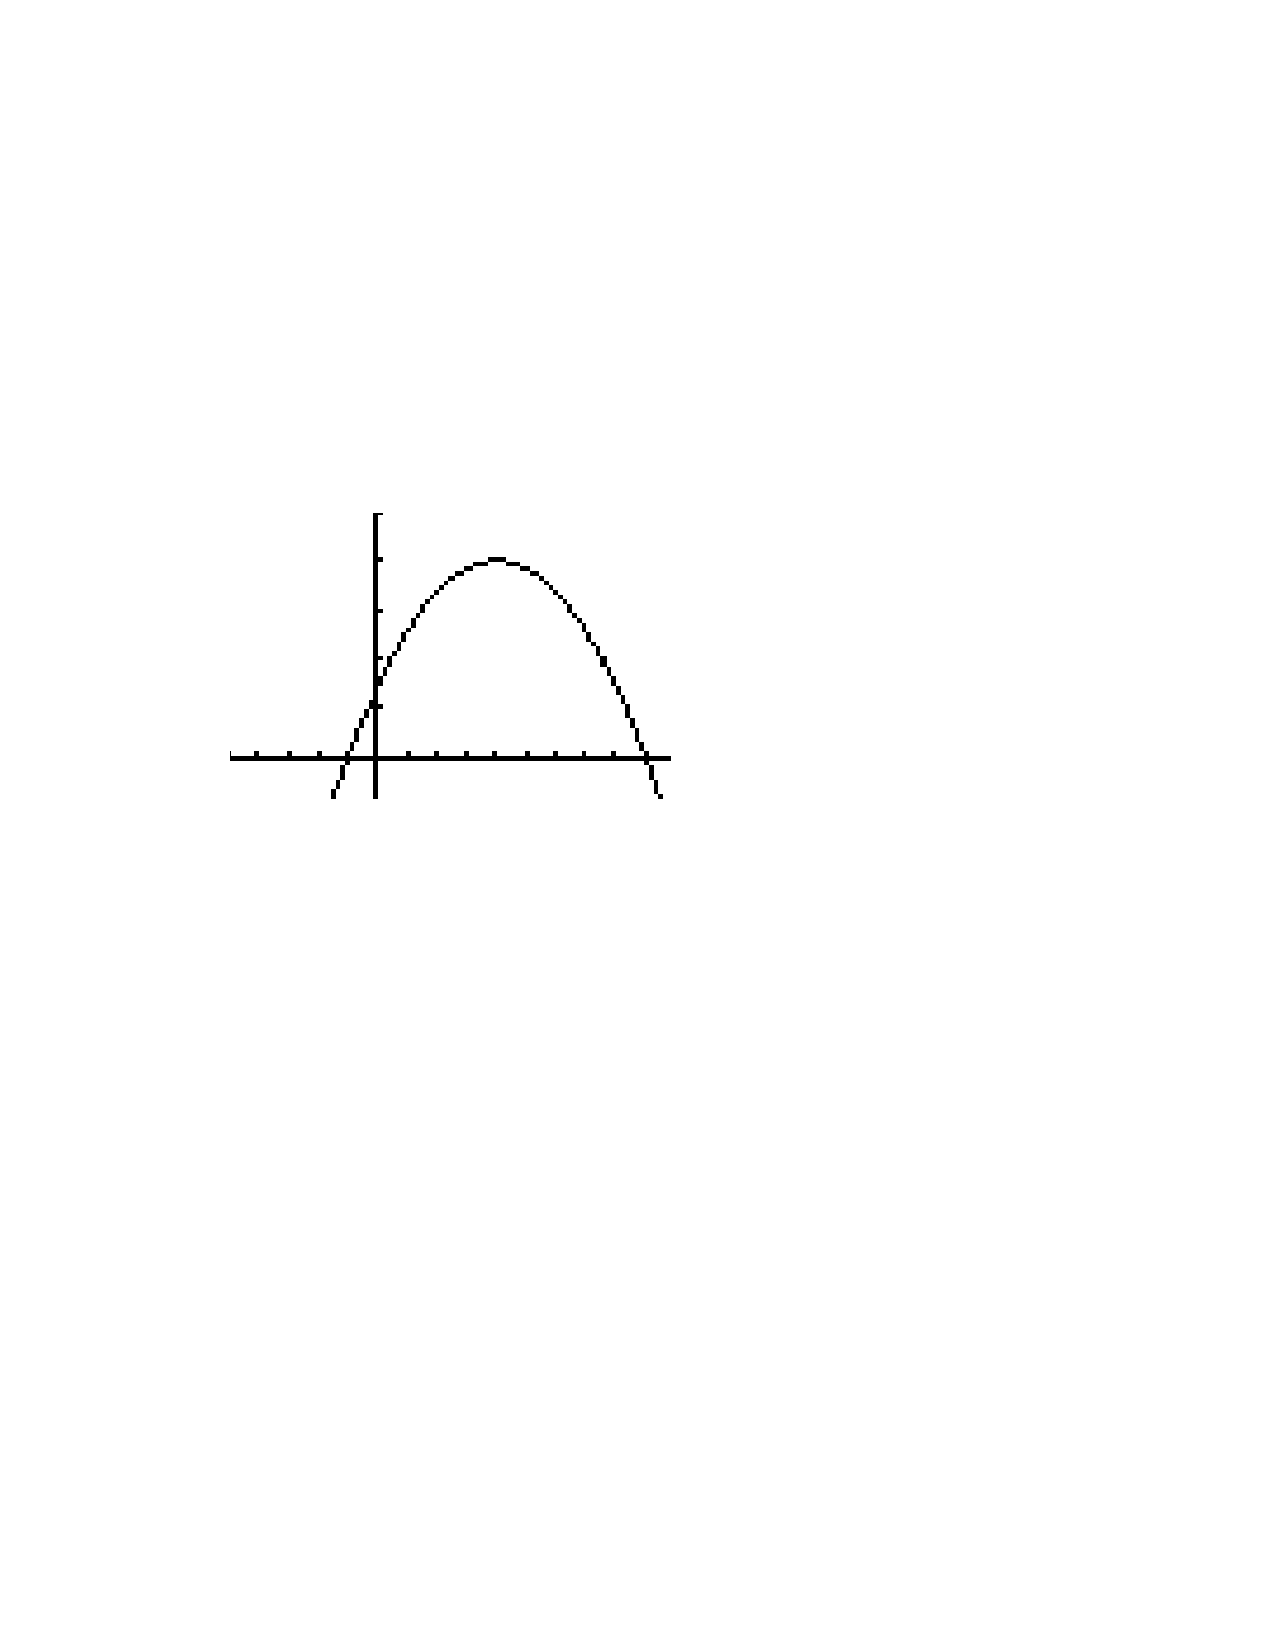
\includegraphics[trim= 100 420 320 160]{Images/Figure1.pdf}
  \end{image}
  \begin{freeResponse}
    The function is continuous on $[-1,6]$ and differentiable on $(-1,6)$: hence it satisfies the hypothesis of the Mean Value Theorem.
    \begin{image}
      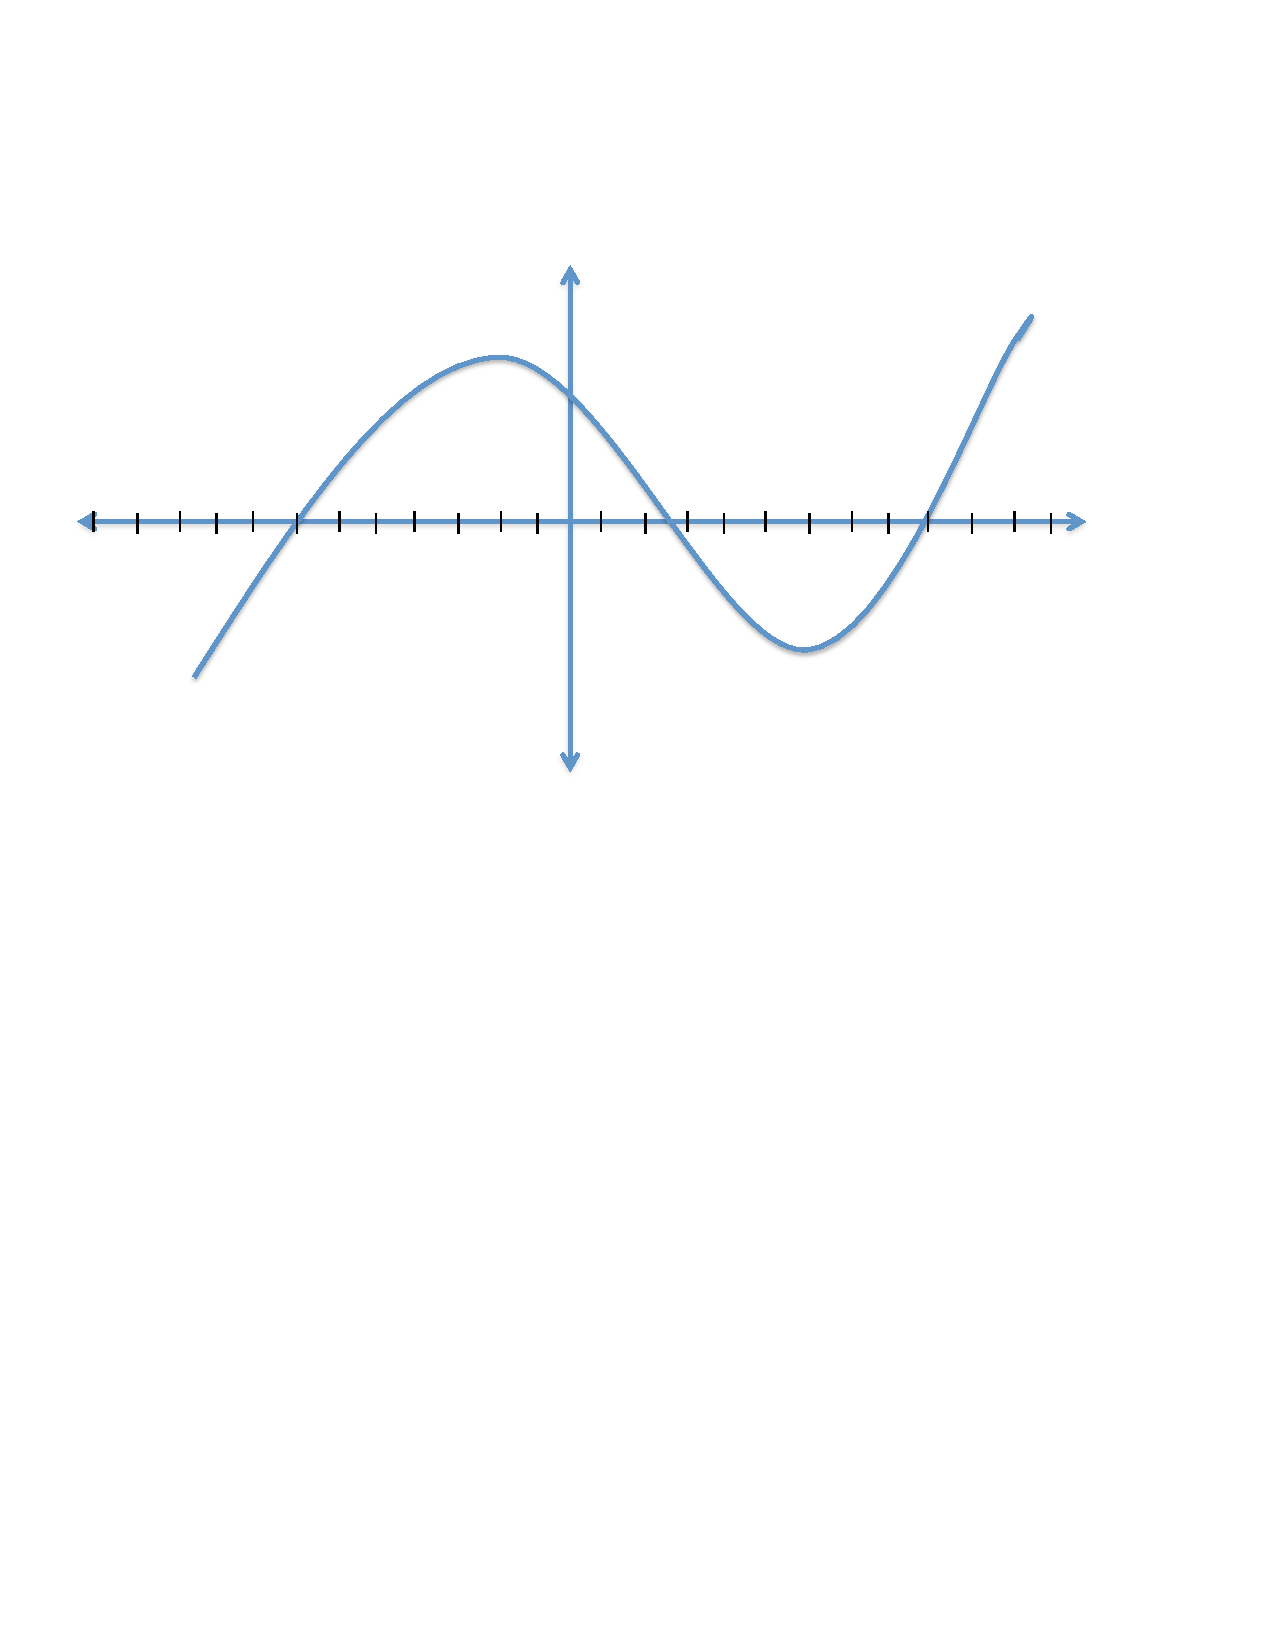
\includegraphics[trim= 100 460 320 190]{Images/Figure2.pdf}
    \end{image}
  \end{freeResponse}
\end{problem}

\begin{problem}
  Verify that the given function satisfies the hypotheses of the Mean Value Theorem in the given interval.
  Then algebraically find all numbers $c$ that satisfy the conclusion of the Mean Value Theorem.
  Using the graph provided, label the point(s) $c$ and sketch the secant line and the tangent line at $c$
  $$ f(x) = \frac{x}{x+2} \qquad \text{on } [1,4] $$.
  \begin{image}
    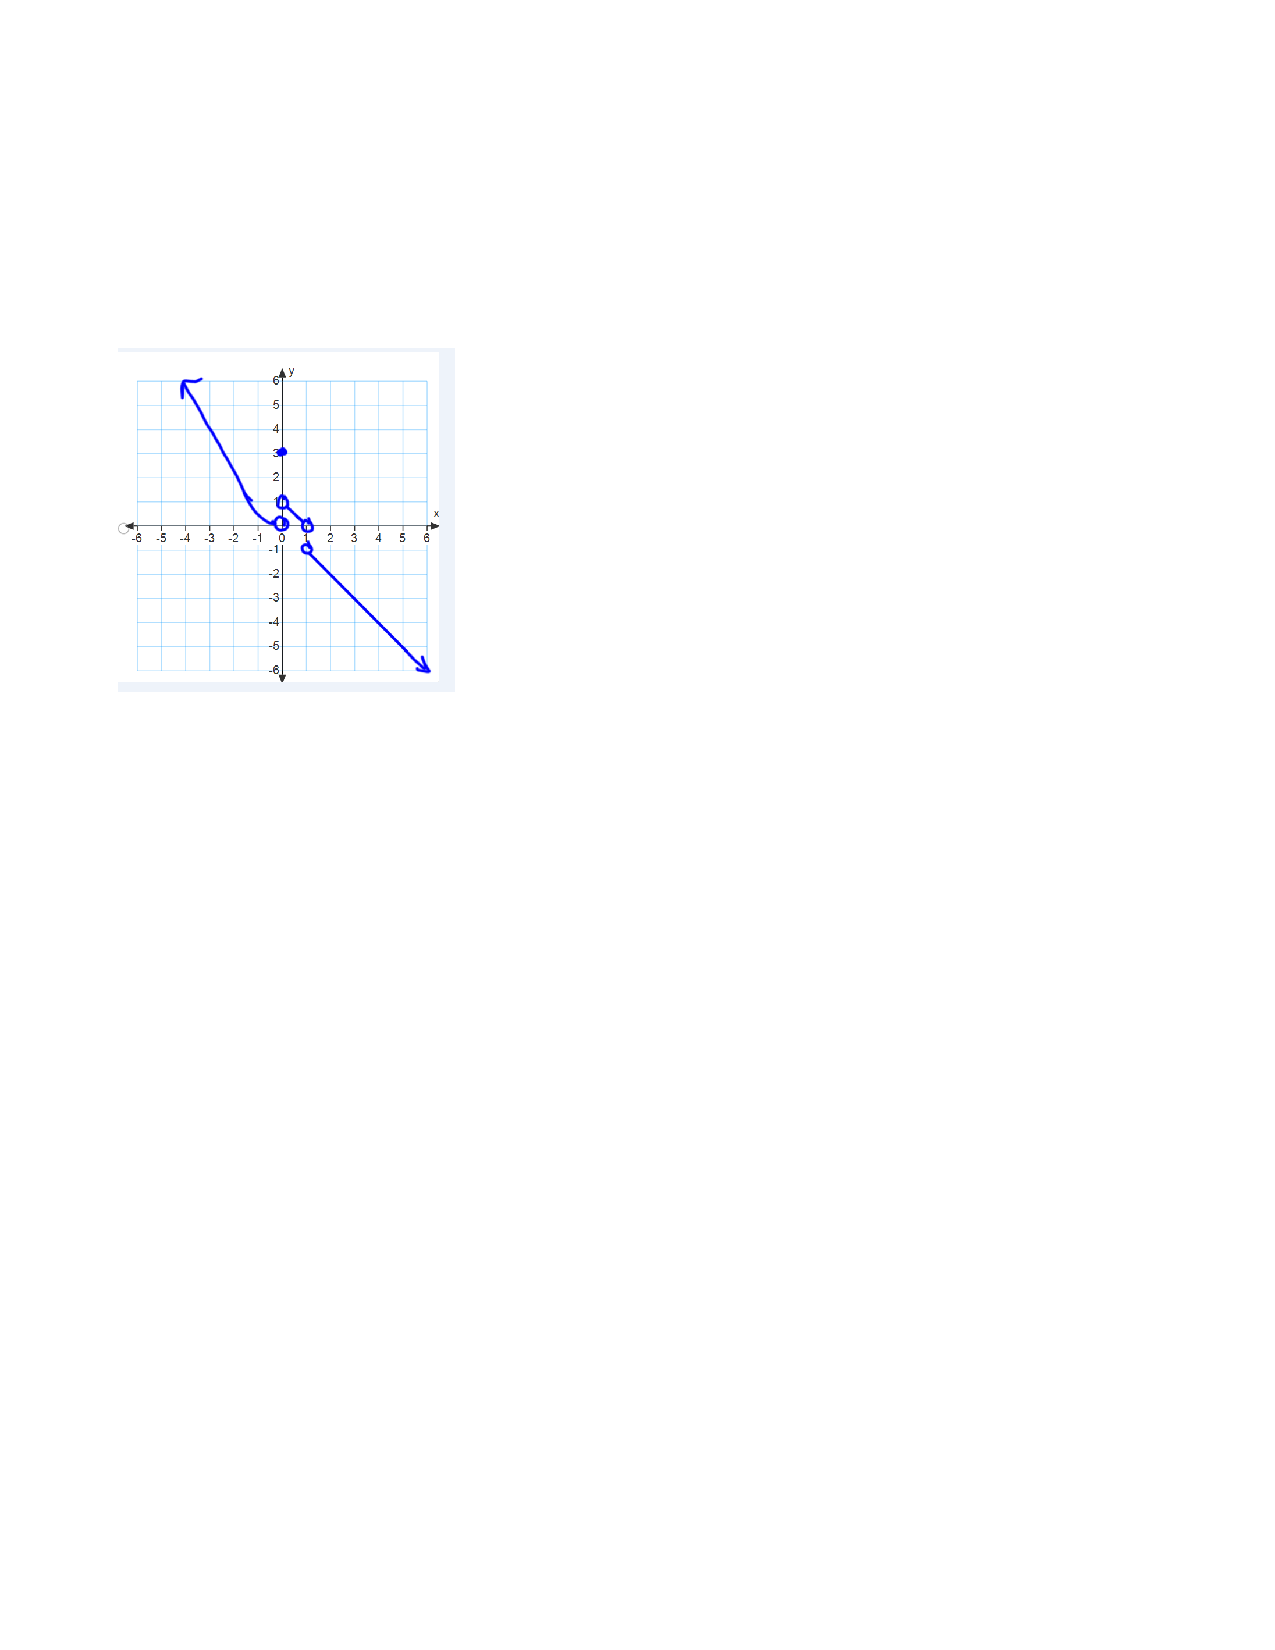
\includegraphics[trim= 120 480 350 180]{Images/Figure3.pdf}
  \end{image}
  \begin{freeResponse}
    The function $f(x) = \frac{x}{x+2}$ is continuous on $[1,4]$ and differentiable on $(1,4)$ since it is a rational function, and is therefore continuous and differentiable on its domain.
    Therefore, $f$ satisfies the hypotheses of the Mean Value Theorem.
    We have that
    $$ f'(x) = \frac{(x+2)(1) - x(1)}{(x+2)^2} = \frac{2}{(x+2)^2} $$
    $$ \frac{f(4) - f(1)}{4-1} = \frac{\frac{2}{3} - \frac{1}{3}}{3} = \frac{1}{9} $$
    So we are looking to find all points $c \in (1,4)$ which satisfy that $ f'(c) = \frac{1}{9} $.  So we solve:
    $$ \frac{2}{(c+2)^2} = \frac{1}{9} $$
    $$ (c+2)^2 = 18 $$
    $$ c = \sqrt{18} - 2 = 3\sqrt{2} - 2 $$
    Note that we omitted $-\sqrt{18} - 2$ above because it is not in the interval $(1,4)$.  Therefore, $c = 3\sqrt{2} - 2$.
    
    \begin{image}
      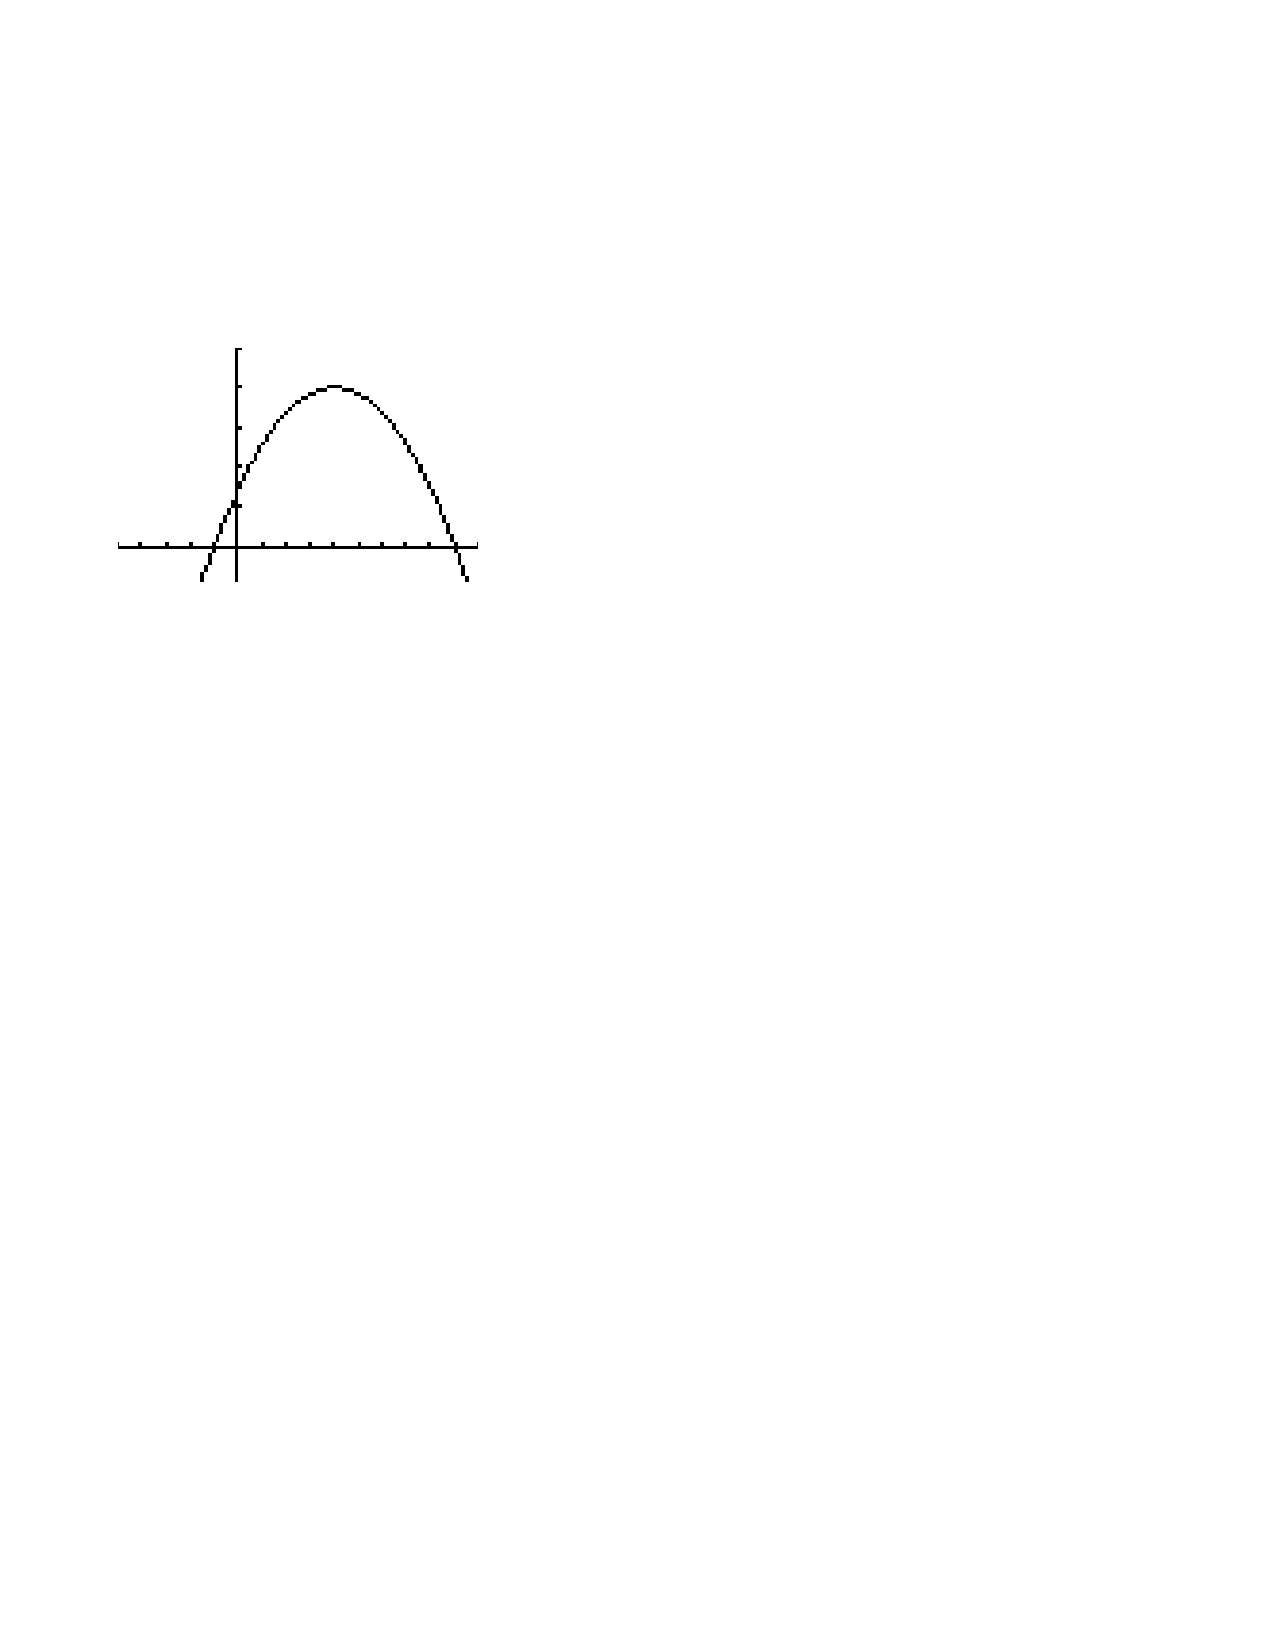
\includegraphics[trim= 130 420 250 180]{Images/Figure4.pdf}
    \end{image}
  \end{freeResponse}
\end{problem}

\begin{problem}
  Let $f(x) = (x-3)^{-2}$.
  Show that there is no value $c$ in $(1,4)$ such that $f(4) - f(1) = f^{\prime}(c) (4-1)$.
  Why does this not contradict the Mean Value Theorem?
  \begin{freeResponse}
    First notice that 
    $$f(4)-f(1) = 1^{-2} - (-2)^{-2} = 1-\frac{1}{4} = \frac{3}{4}$$
    and so we are looking for a value $c$ such that 
    $$3 f^\prime (c) = \frac{3}{4} \quad \Longrightarrow \quad f^\prime (c) = \frac{1}{4} $$
    Then since $f'(x) = \frac{-2}{(x-3)^3}$, we can compute:
    $$ f'(c) = \frac{-2}{(c-3)^3} := \frac{1}{4}$$
    $$ (c-3)^3 = - 8 $$
    $$ c = 3 - 2 = 1 $$
    But $1$ is not in the interval $(1,4)$.  This does not contradict the Mean Value Theorem since $f$ is not continuous at $x=3$.

    \begin{image}
      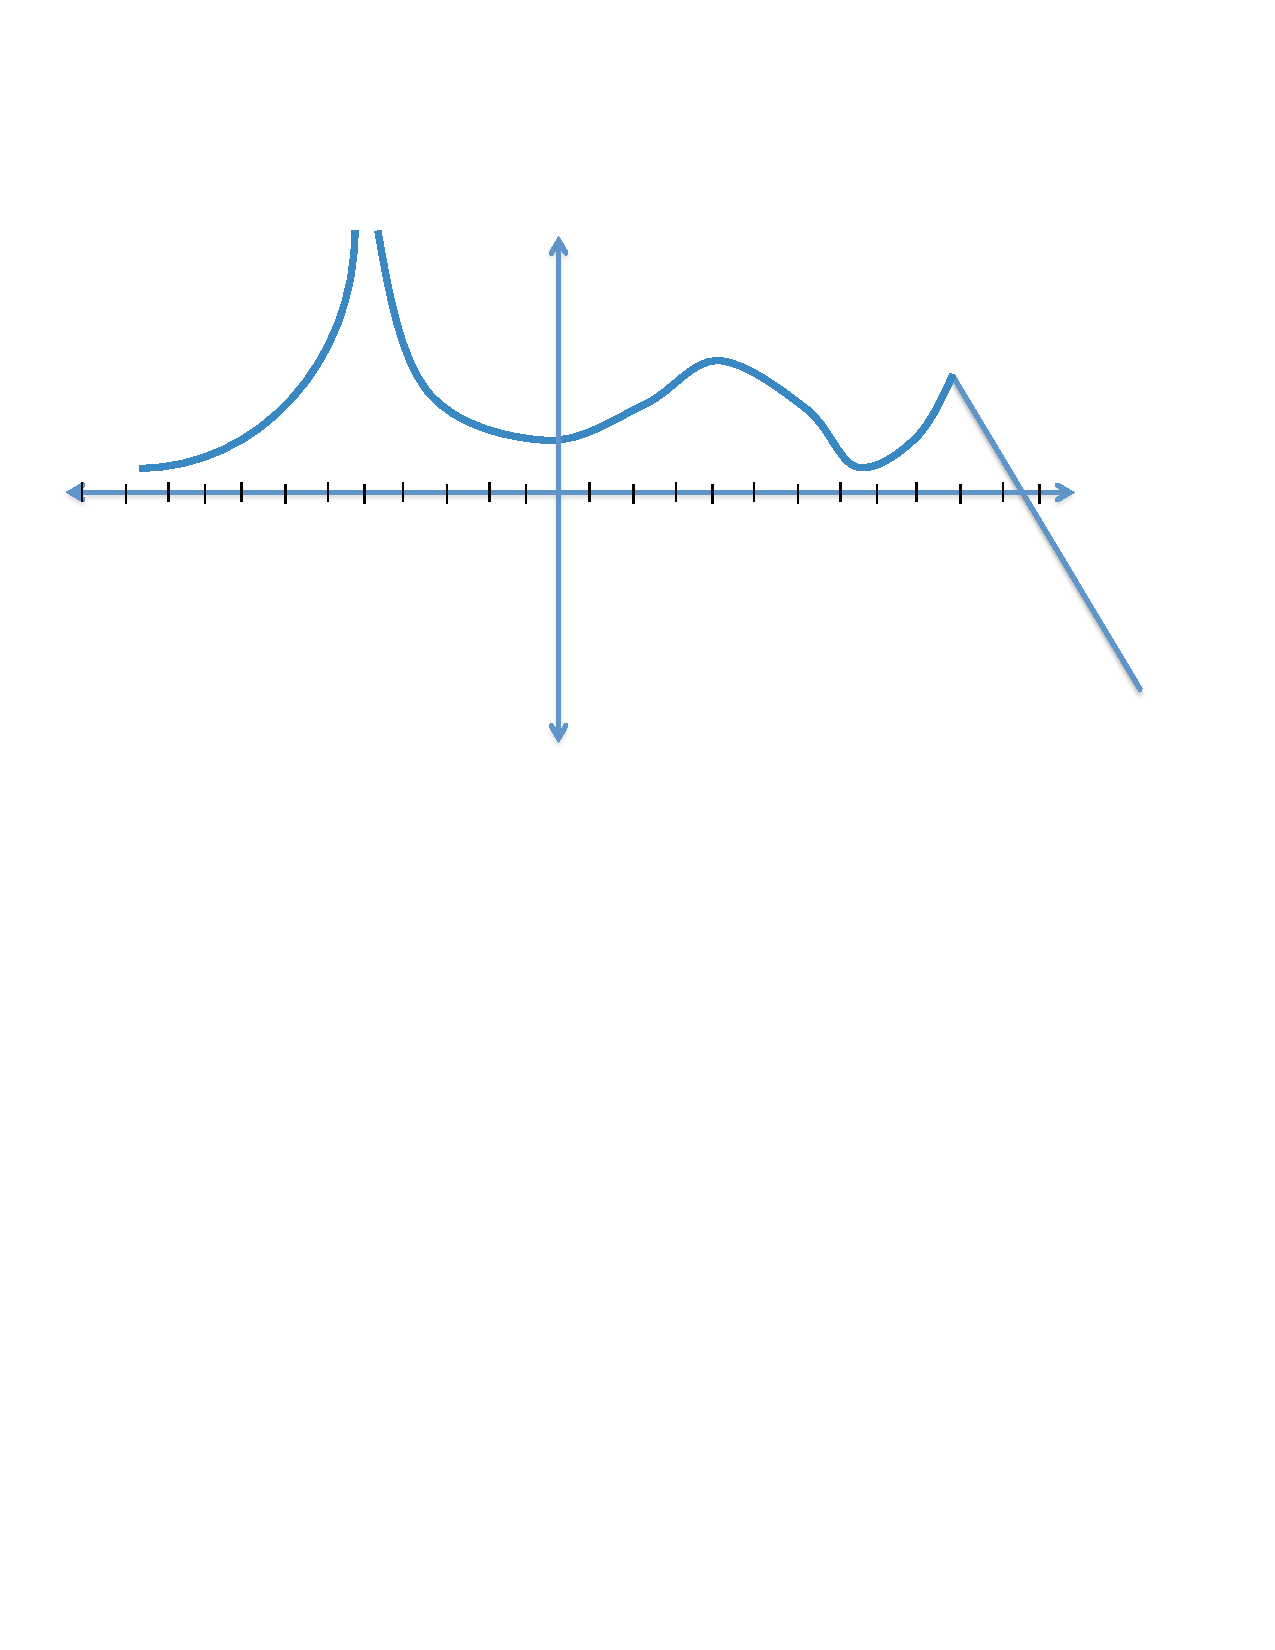
\includegraphics[trim= 100 440 300 210]{Images/Figure5.pdf}
    \end{image}
  \end{freeResponse}
\end{problem}

\begin{problem}
  Two runners start a race at the same time and finish in a tie.
  Prove that at some time during the race they have the same speed.
  (Hint:  Consider the function $h(t)=f(t)-g(t)$, where $f(t)$ and $g(t)$ are the position of the first and second runner at time $t$, respectively.)
  \begin{freeResponse}
    Let $f(t)$ be the position of the first runner at time $t$, and let $g(t)$ be the position of the second runner at time $t$.
    Let $T$ denote the time that the two runners finish the race (which is the same, since they finish in a tie).
    Also, let $h(t) = f(t) - g(t)$.
    Since $h(0) = 0$ and $h(T) = 0$, by Rolle's Theorem there exists some $c$ with $0 < c < T$ such that $h'(c)=0$.
    But since $h^\prime (t) = f^\prime (t) - g^\prime (t)$, we have that $f^\prime (c) = g^\prime (c)$.
    Therefore, the runners hae the same speed at time $c$.  

    \begin{image}
      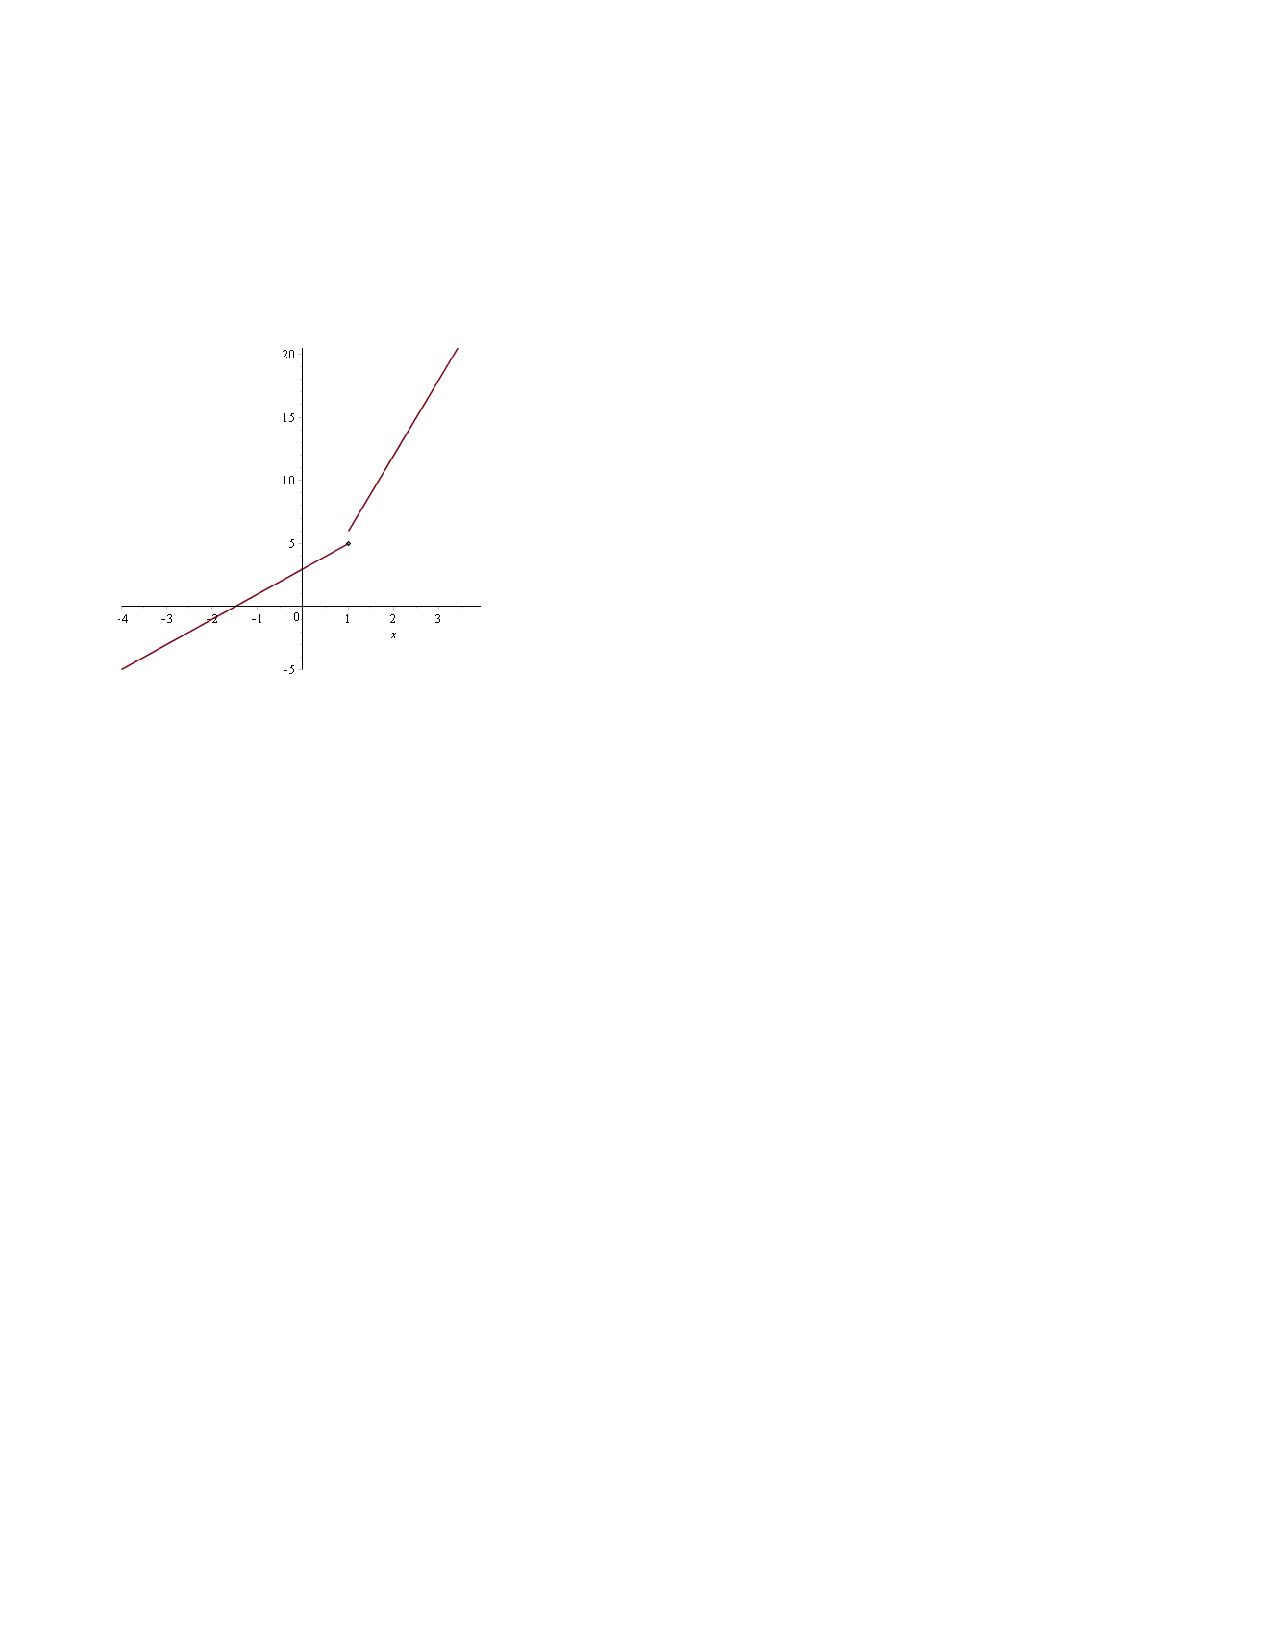
\includegraphics[trim= 100 440 300 180]{Images/Figure6.pdf}
    \end{image}
  \end{freeResponse}
\end{problem}
\end{document} 
